\section{Introduction}

We have interpreted the DNA copy number analysis discussed in \cite{krasnitz2013target} as follows: given possibly overlapping ``defect'' intervals on a line, cover them with a set number of ``explanation'' intervals.  An explanation can only get credit for a defect if the explanation is a subset of said defect.  This is a special case of the maximum coverage problem, where our objective is to maximize the monotone submodular scoring function over a very structured set of subsets.  The hardness of this problem remains an open question.

\subsection{Prior Work} 

While the problem was formulated in relation to the CORE software product in \cite{krasnitz2013target}, the work done on related problems heavily influenced our algorithm development.  Our dynamic programming approach, as well as the definition of maximal explanations, started as an extension of the stabbing problem in \cite{katz2005orthogonal}. 

There is a graph formulation on which a maximum independent set would solve this problem. The heuristic approaches to maximal independent set in \cite{blelloch2012greedy} inspired those graph based approaches and lead directly to the counterexample to our LP relaxation constraint matrix being total unimodular. 

The $k$-OPT approach to maximum clique problem used in \cite{katayama2005effective} as well as previous exposure to the Lin-Kerrigan heuristic \cite{lin1973effective} motivated our own $k$-OPT algorithm.

\section{Description of the problem}

We imagine the genome as an interval graph. The set $D$ contains (possibly overlapping) intervals where damage has been observed.  We seek to find a set of $k$ explanations, $E$ that cover as much of $D$ as possible.

\begin{figure*}[ht!]
    \centering
        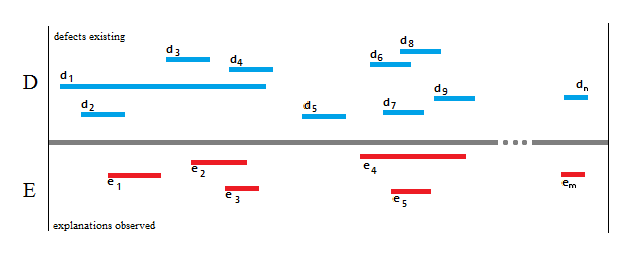
\includegraphics[width=0.99\textwidth]{baseline.png}
    \caption{a general description of the problem.}
\label{fig:genDesc1}
\end{figure*}

An explanation gets 'credit' for an area of overlap of a defect of which is it a proper subset. In figure~\ref{fig:genDesc1}, this means that $e_1$ may be allocated credit for explaining defect $d_1$, but not $d_2$.  The amount of credit for covering a defect is $\frac{ | e_i |}{|d_j|}$, i.e. the fraction of the defect covered by the explanation.
 
When two explanations $e_i,e_j$ overlap and both are a subset of a defect, they may be attributed at most $\frac{ | (e_i \cup e_j) |}{|d_k|}$. For example, in the above diagram, the intersection of $e_2$ and $e_3$ will be attributed as an explanation on $d_1$. They will be given no 'credit' for any explanation of $e_4$, because the segment is not a proper subset of $d_4.$

Goal : Given $k$ explanations, cover the maximum fraction of $D$.

\subsection{Definitions}

For the problem at hand, we have a set of defects $D = \{d_i\}$.  The endpoints of these defects are the integers $l_i, r_i$.  

We have a set of all relevant explanations $E = \{e_1, e_2, ... e_m\}$.  The number of explanations we can use is $k$.

The output explanation set from our algorithm is $A = \{S_1, S_2, ... S_k\}$.  Score($e_i | A$) is the improvement to our score from the explanation $e_i$ given that all of the explanations in $A$ are already in our solution.

The set $T = t_1, t_2, ... t_k$ is the optimal explanation set, i.e. the highest scoring set of $k$ explanations.  Score$(T) = $ OPT.

A {\it defect primitive} $d_{i,j}$ is the portion of defect $d_i$ between the consecutive endpoints $x_j$ and $x_{j+1}$, where $x_j$ and $x_{j+1}$ are the endpoints of any defect in the set.  As all maximal explanations start and end at these endpoint (from Lemma~\ref{lemma:Maximal}), defect primitives are atomic: either they are wholly explained or not explained at all.

\begin{figure}[H] \centering
  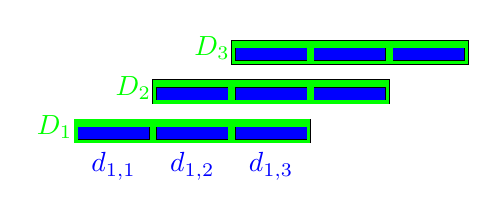
\begin{tikzpicture}[scale=1]

    \foreach \y in {1,2,3} {
      \draw (\y+1, \y/2) rectangle (\y+4, \y/2+.3);
      \fill[green] (\y+1, \y/2) rectangle (\y+4, \y/2+.3);
      \foreach \x in {1,2,3} {
        \draw (\x+\y+.05,\y/2 +.05) rectangle (\x+\y+.95,\y/2+.2);
        \fill[blue] (\x+\y+.05,\y/2 +.05) rectangle (\x+\y+.95,\y/2+.2);
      }
    }

    \foreach \x in {1,2,3} {
      \node[blue] at (1.5+\x,.5) [below] {$d_{1,\x}$};
    }
    
    
    \foreach \x in {1,2,3} {
      \node[green] at (\x+.75,.2+\x/2) {$D_\x$};
    }

  \end{tikzpicture} 
  \caption{{\color{green} Defects} and {\color{blue} defect primitives}.}
  \label{fig:defectPrimitives}
\end{figure}

A primitive's {\it depth} is the number of defects for which it is a subset.  

\subsection{Observation}

The following simplifying observation is useful:

\begin{lem} \label{lemma:Maximal}
Though any interval could be considered for membership in $E$, only ones that share endpoints with members of $D$ are interesting (i.e. candidates for inclusion in the maximal solution).  
\end{lem}

\begin{proof}
First off, explanations that are not proper subsets of any member of $D$ score nothing, so we ignore those.

By contradiction, the explanation $e = [a,b]$ is a proper subset of some number of defects, $G = \cap_i d_i$.  One or more of $a$ and $b$ are not endpoints of a defect.  The credit it gets is $\sum_i \frac{ (b-a) }{|d_i|} $, i.e. proportional to $(b-a)$.

Each $d_i \in G$ can be represented as $[l_i,r_i]$.  We construct the interval $[\max{l_i}, \min{r_i}]$.  Its credit is $\sum_i \frac{ (\min{r_i} - \max{l_i} ) }{|d_i|} $.  

Because $[a,b]$ is a subset of $G$, we know that $\forall_i a \geq l_i, b_i \leq r_i$.  Thus, $\min{r_i} - \max{l_i} \geq b-a$ where the inequality is only tight at $[a,b] = [\max{l_i}, \min{r_i}]$.  This contradicts the assumption that an interesting explanation doesn't share an endpoint with a defect.
\end{proof}

\section{Greedy Algorithm} \label{sec:greedy}

The obvious greedy algorithm would look at all possible explanations that could be placed, and place that explanation. This explanation would score certain portions of one or more defects.  The next step of the greedy algorithm would find the single explanation that scores the best in the presence of the existing solution.  

\begin{algorithm}
  \caption{ \texttt{greedyExplanationCover($D,k$)} }
  \label{alg:greedy}
  \begin{algorithmic}
    \State $M$ = set of maximal explanations
    \State $E = \emptyset$
    \While{ $|E| < k$ }
    \State $e_i = \argmax_{m\in M} S(D,m|E)$
    \State $E \leftarrow E \cup e_i$
    \EndWhile
    \State \Return $E$
  \end{algorithmic}
\end{algorithm}

\subsection{Automated Worst Case Generation}

In order to characterize the worst case performance ratio of \texttt{greedyExplanationCover($D$)}, we decided to first perform a black box analysis of its outputs.  Our methodology was simple: 

\begin{enumerate}
\item For fixed $k$, generate a defect set, $D$
\item Given $D$, compute the greedy explanation set $E$, and its score.
\item Compute optimum score and compare to the greedy score.
\end{enumerate}

To generate the defect endpoints, we randomly choose two integers per defect in the interval $[1,1000]$ and assign the lower (higher) to $l_i$ ($r_i$).  Because the underlying problem is on DNA with discrete base pair positions, integers were judged more appropriate than floating point positions.

Computing the optimum score is trivial for one special case of problems: the set of problems where $k$ = $|D|$.  In such cases, the optimal ouput set is just $D$ and the maximum score is $|D|$.  

\begin{tabular}{l|l}
k & $\frac{Greedy}{OPT}$ \\ \hline
 2 & .750001  \\
 3 & .779596  \\
 4 & .75361   \\
 5 & .800568  \\
 6 & .776081  \\
 7 & .806111  \\
12 & .931058  \\
36 & .995146  \\
\end{tabular}

Our results indicated that we should look at $\frac34$ as the performance ratio of the greedy algorithm.

\subsubsection{Worst Case Analysis}

Our computer simulations showed us scores for which we know cases exist on which greedy does poorly, and it also showed us the defect sets leading to said worst case behavior.  We performed case analysis for $k=2$ and $k=3$ to compare the computer's output with analytic results.

\paragraph{\textbf{$k=2$}} 

\begin{figure}[ht!] \centering
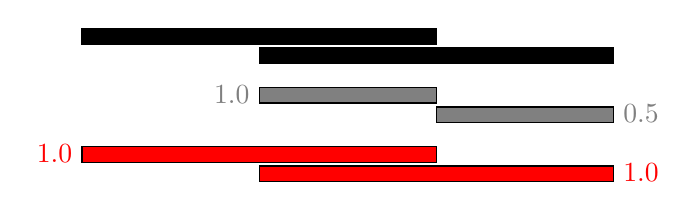
\begin{tikzpicture}[xscale=4.5,yscale=.5]

\fill[black] (0,4) rectangle (1,4.4);
\draw (0,4) rectangle (1,4.4);

\fill[black] (.5,3.5) rectangle (1.5,3.9);
\draw (.5,3.5) rectangle (1.5,3.9);


\fill[gray] (.5,2.5) rectangle (1,2.9);
\draw (.5,2.5) rectangle (1,2.9);
\node[gray] at (.5,3.2) [below left] {1.0};

%  \node[red] at (0,-.8) [above left] {$E_1$};

\fill[gray] (1,2) rectangle (1.5,2.4);
\draw (1,2) rectangle (1.5,2.4);
\node[gray] at (1.5,2.7) [below right] {0.5};

\fill[red] (0,1) rectangle (1,1.4);
\draw (0,1) rectangle (1,1.4);
\node[red] at (0,1.7) [below left] {1.0};

\fill[red] (.5,0.5) rectangle (1.5,0.9);
\draw (.5,0.5) rectangle (1.5,0.9);
\node[red] at (1.5,1.2) [below right] {1.0};

\end{tikzpicture} 
\caption{Worst case for $k=2$ Defects, \textcolor{gray}{Greedy solution} \textcolor{red}{Optimal solution}.  Numbers are scores of the explanation.}
\label{fig:k2}
\end{figure}

The first explanation placed has to score at least one, i.e. $S_1 \geq 1$, since it is the highest scoring explanation and covering either defect scores exactly one.  

For the second explanation, $S_2 \geq \frac{2 - S_1}{2}$.  This follows from a simple pidgeonhole argument: there are at most two defects with some regions uncovered.  The sum of those remaining scores is $2 - S_1$.  The higher scoring of those two defects has to yield at least half of this.  

Combining the two, we get $S_1 + S_2 \geq 1 + \frac{S_1}{2}$, this quantity is at least $\frac32$. 

The defect set in figure~\ref{fig:k2} would be scored $\frac32$ by the greedy algorithm, assuming it made the worst choice at the first step.

\paragraph{\textbf{$k=3$}} 

With 3 defects, we resort to case analysis.  A case will be defined by a table like:

\begin{tabular}{cccc}\hline
Round & Size & Score & Remainder \\ \hline
a & b & c & d \\
\end{tabular}

\begin{tabular}{l}
{\bf Round:} which explanation we're applying. \\
{\bf Size:} number of defects touched this round.  \\
{\bf Score:} score gained this round.  \\
{\bf Remainder:} total unexplained portions. \\
\end{tabular}

\begin{tabular}{cccc}\hline
Round & Size & Score & Remainder \\ \hline
1 & 3 & $\geq 1$ & 2 \\
2 & 1 & $\geq \frac23$ & $\frac43$ \\
3 & ? & $\geq \frac23$ & $\frac23$ \\
\end{tabular}

Where round 2's bound comes from the pigeonhole argument: with 3 total defects, and a score of 2 remaining, one yields at least $\frac23$.  Round 3 is also pigeonhole: in round 2 we completely covered one defect, the remainder of $\frac43$ is shared amongst 2 defects, thus one yields at least $\frac23$.

\begin{tabular}{cccc}\hline
Round & Size & Score & Remainder \\ \hline
1 & 3 & $S_1 \geq 1$ & 2 \\
2 & 2 & $S_2 + S_1 \geq 2$ & 1 \\
3 & ? & $\geq \frac13$ & $\frac23$ \\
\end{tabular}

In round one, we take fractions ${a,b,c}$ from the first, second and third defects.  WOLG, we say that in round 2, the two defects covered are the first and second for fractions $a_2 + b_2 = p$.  We know $a + b + p \leq a + b + c$ since $A \cap B$ wasn't covered in round one.  Thus $p \leq c$.  The remainders of each defect are also less than $p$: 

\begin{eqnarray*}
p \geq (1-a) & \rightarrow a \geq 1-p \\
p \geq (1-b) &\rightarrow b \geq 1-p \\
\end{eqnarray*}

Now we show how round one and two sum to a number greater than two:

\begin{eqnarray*}
S_1 = a+b+c &\geq (1-p) + (1-p) + c \\
S_1 &\geq 2 + c - 2p \\
S_2 &= p \\
S_1 + S_2 &\geq 2 + (c - p) \\
p \leq c &\rightarrow (c-p) \geq 0 \\
S_1 + S_2 &\geq 2 + (0) \\
\end{eqnarray*}

Round three is the standard pigeonhole argument.

\begin{tabular}{cccc}\hline
Round & Size & Score & Remainder \\ \hline
1 & 2 & $\geq 1$ & 2 \\
2 & ? & $\geq 1$ & 1 \\
3 & ? & $\geq \frac13$ & $\frac23$ \\
\end{tabular}

Round 2 has to be at least one since there was an untouched defect entering that round, and any maximum explanation has to score at least that much.  Then round three follows by pigeonhole.

\begin{tabular}{cccc}\hline
Round & Size & Score & Remainder \\ \hline
1 & 1 & $\geq 1$ & 2 \\
2 & ? & $\geq 1$ & 1 \\
3 & ? & $\geq \frac13$ & $\frac23$ \\
\end{tabular}

Exact same argument as above.

\paragraph{Concrete $k=3$ Example}

We've seen that the worst remainder we can achieve for 3 defects being covered with 3 explanations is $\frac23$.  This means greedy will score at least $\frac79$ of optimal.  Note: in figure~\ref{fig:k3}, only one of the three $\frac13$ gray explanations is chosen.

\begin{figure}[ht!] \centering
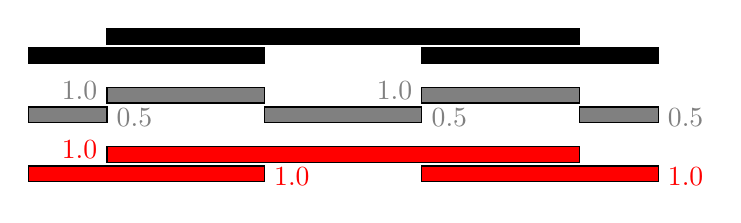
\begin{tikzpicture}[xscale=1,yscale=.5]

\fill[black] (1,4) rectangle (7,4.4);
\draw (1,4) rectangle (7,4.4);

\fill[black] (0,3.5) rectangle (3,3.9);
\draw (0,3.5) rectangle (3,3.9);

\fill[black] (5,3.5) rectangle (8,3.9);
\draw (5,3.5) rectangle (8,3.9);


\fill[gray] (1,2.5) rectangle (3,2.9);
\draw (1,2.5) rectangle (3,2.9);
\node[gray] at (1,3.3) [below left] {1.0};

\fill[gray] (5,2.5) rectangle (7,2.9);
\draw (5,2.5) rectangle (7,2.9);
\node[gray] at (5,3.3) [below left] {1.0};

% 1/3 row
\fill[gray] (0,2) rectangle (1,2.4);
\draw (0,2) rectangle (1,2.4);
\node[gray] at (1,2.6) [below right] {0.5};

\fill[gray] (3,2) rectangle (5,2.4);
\draw (3,2) rectangle (5,2.4);
\node[gray] at (5,2.6) [below right] {0.5};

\fill[gray] (7,2) rectangle (8,2.4);
\draw (7,2) rectangle (8,2.4);
\node[gray] at (8,2.6) [below right] {0.5};

\fill[red] (1,1) rectangle (7,1.4);
\draw (1,1) rectangle (7,1.4);
\node[red] at (1,1.8) [below left] {1.0};

\fill[red] (0,0.5) rectangle (3,0.9);
\draw (0,0.5) rectangle (3,0.9);
\node[red] at (3,1.1) [below right] {1.0};

\fill[red] (5,0.5) rectangle (8,0.9);
\draw (5,0.5) rectangle (8,0.9);
\node[red] at (8,1.1) [below right] {1.0};

\end{tikzpicture} 
\caption{Worst case for $k=3$ Defects, \textcolor{gray}{Greedy solution}, \textcolor{red}{Optimal solution}.  Numbers are scores of the explanation.}
\label{fig:k3}
\end{figure}

\subsubsection{Upper Performance Bound}

It is important to note that the example in figure \ref{fig:k2} can be extended for any even $N$. By placing $\frac{N}{2}$ non-overlapping copies along the number line we create an instance where the first $\frac{N}{2}$ explanations placed by the greedy algorithm score 1 while the next $\frac{N}{2}$ all score $\frac12$.  These sum to $\frac{3N}{4}$ which is clearly $\frac{3}{4}$ of the $N$ that an optimal soution would score.

\subsection{\texttt{MAXIMUM COVERAGE}}

\textit{AKA The $\frac{e-1}{e}$ Barrier}

For \texttt{MAXIMUM COVERAGE}, a related problem, the greedy algorithm is known to have an approximation ratio of  $(1-\frac{1}{e})$.  That is: 

\begin{thm} Given a set $P$ of sets $P_i$, the percentage of the total elements covered by the greedy algorithm can be as bad as $(1-\frac{1}{e})$ times OPT.
\end{thm}

\begin{proof} We define:

\begin{tabularx}{\linewidth}{l X}
{\bf OPT} & The most that can be covered by $k$ subsets. \\
{\bf $x_i$} & Amount covered by greedy in step $i$ \\
{\bf $y_i$} & Total covered by step $i$: $\sum_{j=0}^i x_i$ \\
{\bf $z_i$} & OPT$-y_i$ \\
\end{tabularx}

\begin{lem} \label{lem:MaxPidgeonhole}
For all $i$,  There exists subset where $x_{i+1} \geq \frac{z_i}{k}$.  
\end{lem}

\begin{proof}
Pidgeonhole.  OPT uses $k$ subsets in total.  The residual $z_i$ is no greater than the sum of score remaining in $A^*$, the subsets OPT uses. Since $ |A^*| = k$, one member of $A$ has at least $ \frac{z_i}{k}$ worth of score left. 
\end{proof}

\begin{eqnarray*}
x_{i+1} &\geq \frac{z_i}{k} \\
z_{i+1} &= z_i - x_{i+1} \\
z_{i+1} &\leq z_i - \frac{z_i}{k} = z_i( 1 - \frac{1}{k} ) \\
z_k    &\leq z_0 ( 1 - \frac{1}{k} )^k \\
\lim_{k \rightarrow \infty} ( 1 - \frac{1}{k} )^k &\leq ( 1 - \frac{1}{e}) \\
\lim_{k \rightarrow \infty} z_k &\leq z_0(1 -  \frac{1}{e}) 
\end{eqnarray*}

\end{proof}

\subsection{$k=4$ and Beyond}

After our case analysis and computer simulations, we were convinced that the set coverage greedy approximation factor of $1-\frac{1}{e}$ was overly pessimistic.  Our central contention was that the analysis leading to $1-\frac{1}{e}$ would require at each step for an explanation to hit every single defect.  This is not possible.

\begin{lem} \label{lemma: Number of primitives}
For a set of $n$ defects where all start and end points are unique, if there is one primitive of depth $n$, there is exactly 1, and there are exactly two primitives of each depth between 1 and $n-1$.
\end{lem}

\begin{proof}
This is most easily seen by scanning our endpoints from left to right.  As a left endpoint is reached, our depth increases by exactly one (since only 1 unique endpoint can be reached at once), as a right endpoint is reached, our depth decreases by exactly 1.

We start at depth 0, so to have a primitive of depth $n$, we must scan past exactly $n$ left endpoints and no right endpoints.  As there are only $n$ left endpoints in our defect set, we have exhausted our supply to get a single primitive of depth $n$.

Once we have scanned the first $n$ left endpoints, we passed through exactly $n$ primitives, each of unique depth.  As we continue, we will encounter all $n$ right endpoints.  Each of them will decrease our depth by 1 as we encounter it in our left to right scan, and thus mark the entrance into a new primitive of depths $n-1$, $n-2$, ... 1.  

With one primitive of each depth encountered to the left of our depth $n$ primitive, and another encountered right of our depth $n$ primitive, we have exactly 2 of each depth between 1 and $n-1$.
\end{proof}

Because we can arbitrarially break ties in starting and ending points by judiciously adding powers of $\epsilon$ to actual starting/ending positions, we can treat all defect sets as having unique starting and ending points.  Unfortunately, beyond this observation, we have no bound on how well greedy performs.

\subsection{1-OPT Improvement}

A natural refinement to the greedy algorithm is to improve its output by repeatedly asking whether any of its included explanations can be replaced with an unused explanation to improve the score.  This is known as \texttt{1-OPT} refinement.  

\begin{algorithm}
  \caption{ \texttt{1-OPTExplanationCover($D,k$)} }
  \label{alg:1-OPT}
  \begin{algorithmic}
    \State $E$ =  \texttt{greedyExplanationCover($D,k$)}
    \State haveExchanged = false
    \State $M$ = set of maximal explanations
    \Repeat
    \State haveExchanged = false
    \ForAll{$e_i \in E$}
    \State OldScore = $S(D,E)$
    \State $E' = E / e_i$
    \State $e = argmax_{m \in M} S(D,m|E')$
    \State NewScore = $S(D,e|E')$
    \If{OldScore $< $ NewScore }
    \State haveExchanged = true
    \State $E \leftarrow E' \cup e$
    \EndIf
    \EndFor
    \Until{haveExchanged = false}
    \State \Return $E$
  \end{algorithmic}
\end{algorithm}

In our results section, we will show how much of an imporvement \texttt{1-OPT} was over the greedy algorithm, but here we will show that it does not always lead to the correct answer.

\begin{figure}[h] \centering
    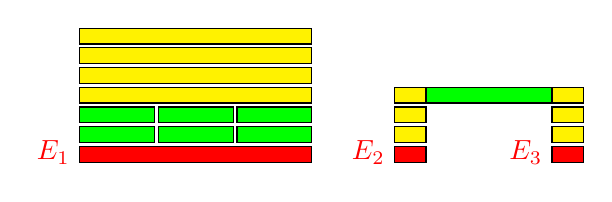
\begin{tikzpicture}[xscale=1,yscale=.5]

      % 6 small rectangles on the left in 2 rows of 3
      \foreach \x in {0,1,2} {
        \foreach \y in {0,1} {
          \fill[green] (0+\x,0+\y/2) rectangle (.95+\x,.4+\y/2);
          \draw (0+\x,0+\y/2) rectangle (.95+\x,.4+\y/2);
        }
      }
      
      % 4 Wide caps on those small rectangles
      \foreach \y in {0,1,2,3} {
        \fill[green] (0,1+\y/2) rectangle (2.95,1.4+\y/2);
        \draw (0,1+\y/2) rectangle (2.95,1.4+\y/2);
      }

      
      \foreach \y in {0,1} {
        \foreach \x in {4, 6} {
          \fill[green] (0+\x,0+\y/2) rectangle (.4+\x,.4+\y/2);
          \draw (0+\x,0+\y/2) rectangle (.4+\x,.4+\y/2);
        }
      }                  

      \fill[green] (4,1) rectangle (6.4,1.4);
      \draw (4,1) rectangle (6.4,1.4);

        \fill[red] (0,-.5) rectangle (2.95, -.1);
        \draw (0,-.5) rectangle (2.95, -.1);
        \node[red] at (0,-.8) [above left] {$E_1$};

        \foreach \y in {0,1,2,3} {
          \fill[yellow] (0,1+\y/2) rectangle (2.95,1.4+\y/2);
          \draw (0,1+\y/2) rectangle (2.95,1.4+\y/2);
        }

        \fill[red] (4,-.5) rectangle (4.4, -.1);
        \draw (4,-.5) rectangle (4.4, -.1);
        \node[red] at (4,-.8) [above left] {$E_2$};
        
        \fill[red] (6,-.5) rectangle (6.4, -.1);
        \draw (6,-.5) rectangle (6.4, -.1);
        \node[red] at (6,-.8) [above left] {$E_3$};

        
        \foreach \y in {0,1,2} {
          \foreach \x in {4, 6} {
            \fill[yellow] (0+\x,0+\y/2) rectangle (.4+\x,.4+\y/2);
            \draw (0+\x,0+\y/2) rectangle (.4+\x,.4+\y/2);
          }
        }                                               
     

    \end{tikzpicture}
    \caption{Initial Greedy Solution}
  \end{figure}          

The initial greedy solution's explanations are red.  It gets full credit for all yellow portions of explanations.  $E_1$ scores 4.  Both $E_2$ and $E_3$ score $2+\epsilon$.  Its score is $8 + 2\epsilon$.

\begin{figure}[h] \centering
  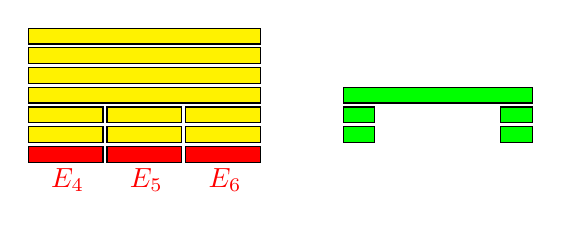
\begin{tikzpicture}[xscale=1,yscale=.5]

    % 6 small rectangles on the left in 2 rows of 3
    \foreach \x in {0,1,2} {
      \foreach \y in {0,1} {
        \fill[green] (0+\x,0+\y/2) rectangle (.95+\x,.4+\y/2);
        \draw (0+\x,0+\y/2) rectangle (.95+\x,.4+\y/2);
      }
    }
    
    % 4 Wide caps on those small rectangles
    \foreach \y in {0,1,2,3} {
      \draw (0,1+\y/2) rectangle (2.95,1.4+\y/2);
      \fill[green] (0,1+\y/2) rectangle (2.95,1.4+\y/2);
    }

    
    \foreach \y in {0,1} {
      \foreach \x in {4, 6} {
        \fill[green] (0+\x,0+\y/2) rectangle (.4+\x,.4+\y/2);
        \draw (0+\x,0+\y/2) rectangle (.4+\x,.4+\y/2);
      }
    }                  

    \fill[green] (4,1) rectangle (6.4,1.4);
    \draw (4,1) rectangle (6.4,1.4);

    \foreach \x in {4,5,6} {
      \fill[red] (-4+\x,-.5) rectangle (-3.05+\x,-.1);
      \draw (-4+\x,-.5) rectangle (-3.05+\x,-.1);
      \node[red] at (-3.5+\x,-1.5) [above] {$E_\x$};
    }

    \foreach \x in {0,1,2} {
      \foreach \y in {0,1} {
        \fill[yellow] (0+\x,0+\y/2) rectangle (.95+\x,.4+\y/2);
        \draw (0+\x,0+\y/2) rectangle (.95+\x,.4+\y/2);
      }
    }
    \foreach \y in {0,1,2,3} {
      \fill[yellow] (0,1+\y/2) rectangle (2.95,1.4+\y/2);
      \draw (0,1+\y/2) rectangle (2.95,1.4+\y/2);
    }
    
  \end{tikzpicture}
  \caption{Optimal Solution}
\end{figure}    

Each of $E_4, E_5, E_6$ score $3 \frac13$ for a total of 10.  

There is no single exchange from the greedy solution with any of the explanations in the optimal solution that improve the score.  Thus \texttt{1-OPT} is a useful refinement, but does not optimally solve the problem.

\texttt{$m$-OPT} refinement is the natural generalization when we ask if any set of $m$ explanations in the current solution can be replaced with another $m$ unused explanations to improve the score.  

\section{Dynamic Programming} \label{sec:DP}

A simple dynamic programming approach, where we score the $k+1$st defect and place all of them between points $a$ and $b$ such as $S(k+1,a,b) = \max_y S(k,a,y) + S(1,y,b)$ fails because the score, $ S(1,y,b)$, is dependent on the full state of which explanations are already placed.

Simply put, the barrier between solved and unsolved regions doesn't exist.

To get around this complication, we've proposed constant depth dynamic programming solutions.  Such a solution is characterized by the maximum number of explanations that can overlap at any one place in the solution.  A depth 1 dynamic programming solution would have no overlaps, and a depth 2 solution can have many regions where 2 explanations overlap, but none where 3 overlap.

\subsection{Depth 1 Dynamic Program} \label{sec:1DP}

A depth 1 dynamic program will find the set of explanations that cover any set of defects with the guarantee that no explanations will overlap.  The recurrence relation is simple: $S(k+1,0,x)$ = $\max_y S(k,0,y) + S(1,y,x)$.  The score we can achieve with $k+1$ explanations in the region $[0,x]$ is the max over intermediary points, $y$, of the score achieved before $y$ with $k$ explanations plus the score we can achieve to the right of $y$ with 1 explanation. The barrier between the completed subproblem and the unsolved region is the point $y$. We cannot place new explanations that start to the left of it.

The obvious question is: how well does this perform compared to an optimal solution which can overlap arbitrarially?

We will construct a non-overlapping solution, compare its value to OPT and then appeal to the correctness of a dynamic programming solution to claim that it will do this well or better.

To construct our solution, we will take OPT as an input.  The $k$ explanations of opt have associated with them $2k-1$ {\it explanation primitives}.  These are  {\it primitives} whose endpoints come from a set of explanations. There are $2k-1$ of them because no more than $2k$ unique points are required to describe $k$ defects.

Were we to use all of OPT's $2k-1$ explanation primitives, we would cover all defects that OPT covers.  If we select the $k$ highest scoring of these explanation primitives, we cover at least half of OPT's total credit. Unfortunately, this is worse than our greedy bound of $(1- \frac{1}{e})$.

\subsection{Depth $d$ Dynamic Program} \label{sec:dpFixedDepth}

For dynamic programs of depth $d \geq 2$, our state is slightly more complicated than it was for depth 1. We have $k$, the number of explanations used, $a$ the end of the solved region, $b$ the end of the active region and $S$, the left endpoints of the set of explanations that are active (there are up to $k$ of them) at point $b$ to form $DS(k,a,b,S)$.


\begin{figure}[ht!] \centering
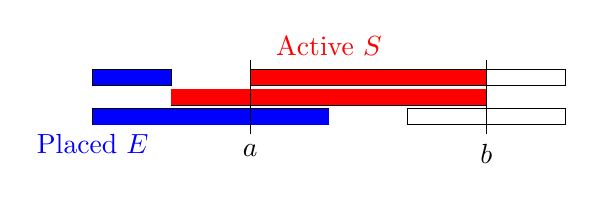
\begin{tikzpicture}[xscale=1,yscale=.25]

\draw (4,0) rectangle (6,0.8);

\draw (1,1) rectangle (5,1.8);
\fill[red] (1,1) rectangle (5,1.8);

\node[red] at (3,3) [above] {Active $S$};

\draw (2,2) rectangle (6,2.8);
\fill[red] (2,2) rectangle (5,2.8);

\draw (0,0) rectangle (3,0.8);
\fill[blue] (0,0) rectangle (3,0.8);

\draw (0,2) rectangle (1,2.8);
\fill[blue] (0,2) rectangle (1,2.8);

\node[blue] at (0,0) [below] {Placed $E$};


\draw (2,-.5) -- (2,3.3);
\node[black] at (2,-.5) [below] {$a$};

\draw (5,-.5) -- (5,3.3);
\node[black] at (5,-.5) [below] {$b$};

\end{tikzpicture} 
\caption{An illustration of a depth $d \geq 3$ DP in action.}
\label{fig:dpIllustration}
\end{figure}

\FloatBarrier

{\bf Running Time:} The memoization table can contain every legal state of the form $DS(k,a,b,S)$.  The first argument takes all values from 0 to $k$ inclusive.  The next two will only hold the values of endpoints, of which there are $2N$ of.  Each member of $S$ can be empty or hold the value of an endpoint, and there can be no more than $k$ members.  This gives us a total running time of: $O(kn^{2+k})$.

In order to build an optimal coverage that never exceeds a depth of $d$, the dynamic program sweeps.  Starting with $a$ and $b$ at the leftmost endpoint, we move them right respecting that $a \leq b$.  An explanation $(L,R)$ can become active iff $L\leq a$ and $R \geq b$ and $|S|<d$ for the current set $S$.

Each state $DS(k,a,b,S)$ has an associated explanation set $E$, the explanations that were placed earlier in the sweep and to attain the maximum current score for our state.  The following four transformations are sufficient to get from any starting state to any final state.

$ DS(k-1,a,b,S-e) \rightarrow DS(k,a,b,S)${\it A new explanation becomes active.} An explanation starting at $e$, where $e > x \forall x \in S$, is added to our active list.

$ DS(k,a-1,a,S + (x,a)) \rightarrow DS(k,a,b,S)${\it An active explanation ends.}  Note the differing endpoints.  If we leave the ending explanation in the active region, it will be able to influence our current scoring region. Thus the active region moves to the right of the departing explanation.

$DS(k,a-1,b,S) \rightarrow DS(k, a, b, S )${\it Left boundary of active region contracts.} Since all explanations in $S$ start and end outside of $[a,b]$, this will not change the obtainable score.  It will, however, disqualify some candidates from joining the set $S$.

$DS(k,a,b-1,S) \rightarrow DS(k, a, b, S )${\it Right boundary of active region expands.} All active explanations in $S$ are treated as having $b$ as their right endpoint until they cease to be active.  Because of that, this movement can lead to explanations in $S$ to become non-scoring and is not always permitted.

\begin{lem} \label{lem:dpCorrect}
Using the rules outlined above, any legal explanation set could be reached.
\end{lem}

\begin{proof}
If we start any legal explanation set $E$ and convert it into the set of sorted endpoints $x_i$, the following sequence (in reverse) would find that set $E$.  

Start with $DS(k,x_k,x_k,\emptyset)$.  Use the ``active explanation ends'' rule  in reverse to get to the state: $DS(k,x_k,x_k,{x^L_k})$ where $x^L_k$ is the left endpoint of the explanation ending at $x_k$.

We can then use the left endpoint moving rule in reverse to get to $DS(k,x_{k-1},x_k,{x^L_k})$ and the right endpoint in reverse to get to $DS(k,x_{k-1},x_{k-1},{x^L_k})$.

If this is the right endpoint of an explantion, we will either use the ``active explanation ends'' as above.  If left, the ``new explanation becomes active'' rule in reverse will take us to the new predecessor state $DS(k-1,x_k,x_k,S_i \setminus{x^L_i} )$.

We would then continue shifting endpoints to $x_{i-1}$ and selecting the appropriate endpoint rule until we reach the leftmost extent of $E$.  With this construction, the members of $S_i$ at $x_i$ are those explanations stabbed by a line through that point.  Since the explanation set's depth is less than $d$, $|S_i|$ will also be less than $d$.  Thus these steps are all legal.
\end{proof}

\subsection{Quality of $d=2$ DP Solution}

Our result from section~\ref{sec:1DP} tells us that a depth 2 dynamic program will score no worse than the $\frac12$ of OPT that a depth 1 dynamic program will.  We can generalize that proof to find tighter bounds.

\begin{lem} \label{lem:2DP2/3}
Each of the $\frac{k}{2}$ subproblems formed by dividing an optimal solution after every fourth explanation primitive can have $65.5\%$ of its optimal score achieved with the use of 2 explanations.
\end{lem}

We prove this by exhaustively enumerating all possible 4 width subproblems, dismissing most of them with a counting argument and then exhaustively covering the remaining two with two explanations and finding the worst case behavior.

The border between any two explanation primitives occurs when an explanation is either ending or starting.  There are exactly three internal borders in any width four subproblem.  We will label classes of similar problems by the events they contain.  Using $1$ to represent a beginning, and $0$ an end, there are 8 naive classes of subproblems: $000, 001, 010 ... 111$.

Mirror image subproblems can be covered with mirror image explanations, and the mirror image of subproblem $abc$ is $\neg c \neg b \neg a$.  This leaves us with four distinct subproblem classes: $110, 101, 111, 011$. 

\subsubsection{Trivial Classes}

The first two classes, $110, 101$ can be drawn in multiple ways depending on which defect the $0$ terminates.  

\begin{figure}[h] \centering 
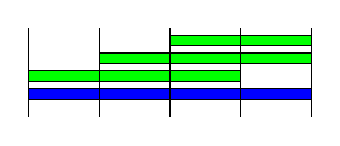
\begin{tikzpicture}[scale=.9]


\fill[blue] (0,.05) rectangle (4,.20);
\draw (0,.05) rectangle (4,.20);

\fill[green] (0,.30) rectangle (3,.45);
\draw (0,.30) rectangle (3,.45);

\foreach \x in {2,3} {
  \fill[green] (\x-1,\x/4 +.05) rectangle (4,\x/4+.20);
  \draw (\x-1,\x/4 +.05) rectangle (4,\x/4+.20);
}

\foreach \x in {0,1,2,3,4} {
    \draw (\x,-.2) -- (\x,1.05);
}


\end{tikzpicture} 
\caption{Class 110a}
\end{figure}

\begin{figure}[h] \centering 
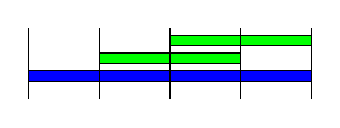
\begin{tikzpicture}[scale=.9]


\fill[blue] (0,.05) rectangle (4,.20);
\draw (0,.05) rectangle (4,.20);

\fill[green] (1,.30) rectangle (3,.45);
\draw (1,.30) rectangle (3,.45);

\fill[green] (2,.55) rectangle (4,.70);
\draw (2,.55) rectangle (4,.70);
 
\foreach \x in {0,1,2,3,4} {
    \draw (\x,-.2) -- (\x,.8);
}


\end{tikzpicture} 
\caption{Class 110b}
\end{figure}

\begin{figure}[h] \centering 
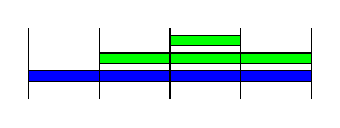
\begin{tikzpicture}[scale=.9]


\fill[blue] (0,.05) rectangle (4,.20);
\draw (0,.05) rectangle (4,.20);

\fill[green] (1,.30) rectangle (4,.45);
\draw (1,.30) rectangle (4,.45);

\fill[green] (2,.55) rectangle (3,.70);
\draw (2,.55) rectangle (3,.70);
 
\foreach \x in {0,1,2,3,4} {
    \draw (\x,-.2) -- (\x,.8);
}

\end{tikzpicture} 
\caption{Class 110c}
\end{figure}

All of the $110$ class members can be completely covered using as explanations the three green defects.  Since we are allowed to choose the two highest scoring of those three, clearly $\frac23$ of the optimal score is trivial for this class. The 101 class is smaller and similarly covered:

\begin{figure}[h] \centering 
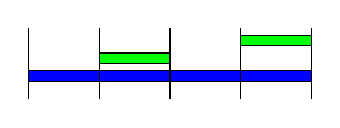
\begin{tikzpicture}[scale=.9]


\fill[blue] (0,.05) rectangle (4,.20);
\draw (0,.05) rectangle (4,.20);

\fill[green] (1,.30) rectangle (2,.45);
\draw (1,.30) rectangle (2,.45);

\fill[green] (3,.55) rectangle (4,.70);
\draw (3,.55) rectangle (4,.70);
 
\foreach \x in {0,1,2,3,4} {
    \draw (\x,-.2) -- (\x,.8);
}


\end{tikzpicture} 
\caption{Class 101a}
\end{figure}

\begin{figure}[h] \centering 
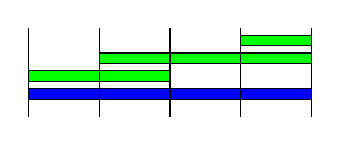
\begin{tikzpicture}[scale=.9]


\fill[blue] (0,.05) rectangle (4,.20);
\draw (0,.05) rectangle (4,.20);

\fill[green] (0,.30) rectangle (2,.45);
\draw (0,.30) rectangle (2,.45);

\fill[green] (1,.55) rectangle (4,.70);
\draw (1,.55) rectangle (4,.70);
 
\fill[green] (3,.80) rectangle (4,.95);
\draw (3,.80) rectangle (4,.95);
 
\foreach \x in {0,1,2,3,4} {
    \draw (\x,-.2) -- (\x,1.05);
}


\end{tikzpicture} 
\caption{Class 101b}
\end{figure}

As with the $110$ class, the members of $101$ can both be covered completely with 3 explanations, meaning 2 can always score $\frac23$ of the optimum score.

\subsubsection{Exhaustive Explanation Enumeration} \label{sec:exhaustiveEnumeration}

The next two classes can each only be drawn in one way and require some labeling and reasoning to get our $.655$ approximation factor.

\begin{figure}[h] \centering 
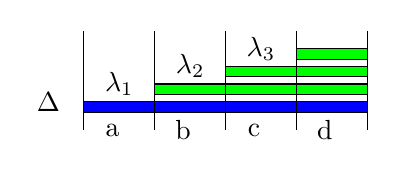
\begin{tikzpicture}[scale=.9]

\foreach \x in {0,1,2,3} {
    \fill[green] (\x,\x/4 +.05) rectangle (4,\x/4+.2);
    \ifnum \x = 0
      \fill[blue] (\x,\x/4 +.05) rectangle (4,\x/4+.2);
    \fi
    \draw (\x,\x/4 +.05) rectangle (4,\x/4+.2);

    \draw (\x,-.2) -- (\x,1.2);
}
\draw (4,-.2) -- (4,1.2);

\node (a) at (0+.4,-.2) {a};
\node (b) at (1+.4,-.2) {b};
\node (c) at (2+.4,-.2) {c};
\node (d) at (3+.4,-.2) {d};

\node (delta) at ( -.5,.2) {$\Delta$};
\node (l1)    at (.5,.45 ) {$\lambda_1$};
\node (l2)    at (1.5,.7 ) {$\lambda_2$};
\node (l3)    at (2.5,.95) {$\lambda_3$};

\end{tikzpicture} 
\caption{Class 111}
\end{figure}

\begin{figure}[h] \centering 
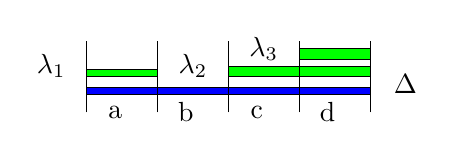
\begin{tikzpicture}[scale=.9]


\fill[blue] (0,.05) rectangle (4,.15);
\draw (0,.05) rectangle (4,.15);

\fill[green] (0,.30) rectangle (1,.40);
\draw (0,.30) rectangle (1,.40);

\foreach \x in {2,3} {
  \fill[green] (\x,\x/4 -.2) rectangle (4,\x/4-.05);
  \draw (\x,\x/4 -.2) rectangle (4,\x/4-.05);
}

\foreach \x in {0,1,2,3,4} {
    \draw (\x,-.2) -- (\x,.8);
}

\node (a) at (0+.4,-.2) {a};
\node (b) at (1+.4,-.2) {b};
\node (c) at (2+.4,-.2) {c};
\node (d) at (3+.4,-.2) {d};

\node (delta) at (4.5,.2 ) {$\Delta$};
\node (l1)    at (-.5,.45) {$\lambda_1$};
\node (l2)    at (1.5,.45) {$\lambda_2$};
\node (l3)    at (2.5,.70) {$\lambda_3$};

\end{tikzpicture} 
\caption{Class 011}
\end{figure}

The full score available from covering a subproblem of class $111$ is:

\begin{align*} 
S_{MAX} = &a \Delta + b \Delta + c \Delta + d \Delta + \hdots \\
& b \lambda_1 + c\lambda_1 + d\lambda_1 + \hdots \\
& c \lambda_2 + d \lambda_2 + d \lambda_3
\end{align*}

The set of maximal explanations for a subproblem of class $111$ would include all explanations that begin where a defect begins and end where one ends.  That set is: $ (0,4) (1,4) (2,4) (3,4)$.  There are $(^4_2) = 6$ possible explanation pairs to cover this region, and so we form a table.

The table, $C$ is $6 \times 10$, with each column representing one of our 6 possible explanation pairs, and each row corresponging to a term in the $S_{MAX}$ sum.  If $C(i,j) = 0$, neither of the explanations in pair $i$ covers term $j$ in the sum. Otherwise, $C(i,j) = 1$.

\begin{tabular}{l|llllll}
      & (0,4) & (0,4) & (0,4) & (1,4) & (1,4) & (2,4) \\
$s_j$ & (1,4) & (2,4) & (3,4) & (2,4) & (3,4) & (3,4) \\ \hline
$a\Delta$ & 1 & 1 & 1 & 0 & 0 & 0 \\
$b\Delta$ & 1 & 1 & 1 & 1 & 1 & 0 \\
$c\Delta$ & 1 & 1 & 1 & 1 & 1 & 1 \\
$d\Delta$ & 1 & 1 & 1 & 1 & 1 & 1 \\
$b \lambda_1$ & 1 & 0 & 0 & 1 & 1 & 0 \\
$c \lambda_1$ & 1 & 1 & 0 & 1 & 1 & 0\\
$d \lambda_1$ & 1 & 1 & 1 & 1 & 1 & 0 \\
$c \lambda_2$ & 0 & 1 & 0 & 1 & 0 & 1\\
$d \lambda_2$ & 0 & 1 & 1 & 1 & 0 & 1\\
$d \lambda_3$ & 0 & 0 & 1 & 0 & 1 & 1\\
\end{tabular}

For any column $i$, the score obtained by placing those two explanations is $\sum_j s_j C(i,j)$.  Because each $s_j$ is a product of $x \in \{ \delta \lambda_1, \lambda_2, \lambda_3 \}$ and $\alpha \in \{ a, b, c, d \}$, our problem can be reformulated as the quadratically constrained quadratic program (QCQP):

\begin{alignat*}{2}
  \text{minimize } & F \\
  \text{ subject to: } & \forall_j F \geq \sum_j s_j C(i,j) \\
                        & \sum_i s_i = 1 \\
                        & \sum_j \alpha_j = 1 \\
                        & \forall_{i>0} x_i \leq 1 \\
                        & 0 < \alpha_i < 1 \\
                        & 0 < x_i \\
\end{alignat*}

Our first constraint ensures that we are minimizing the highest score attainable by any legal combination of maximal explanations. The second constraint, $\sum_i s_i = 1$ scales the score we achieve in this interval, making $F$ the ratio of score we can get to score possible in this interval. The third constraint, $\sum_j \alpha_j = 1$ scales distance to allow for a unique solution to be found.  

The fourth constraint, $\forall_{i>0} x_i \leq 1$ guarantees that each defect $\lambda_k$ can only schieve a score of 1, with the exception of $\delta$. Since $\delta$ represents the sum of all defects that started before this span and end after it, it clearly should not be constrained.

For $d=2$, this QCQP can easily be typed into a computer algrbra system (i.e. Mathematica) or modeling language (like AMPL) and yields a solution of .705 for class $011$ and .655 for $111$.  As we are looking for the worse performing class, we see that in each 4 width subdivision, 2 explanations can score at least $65.5\%$ of the available score.

For $d > 2$, the process outlined in section~\ref{sec:exhaustiveEnumeration} is difficult to do by hand.  We wrote a computer program to solve this problem. Its subroutines:

\begin{enumerate}
\item Given the input $d$, generate all subproblem classes as $2d-1$ bit numbers.  (i.e. $111, 101$)
\item For each class, enumerate all possible matchings of defect beginning and defect end to find all members of a class. (i.e. $101a, 101b$)
\item Check if any set of $d+1$ explanations completely covers the class (since $\alpha$ is theorized to be $\leq \frac{d}{d+1}$).
\item For each of these class members, find the set $|E|$ of maximal explanations.  
\item Using quadratic programming, calculates the min-max of the score of $(^{|E|}_{\hspace{3pt}d})$ of these explanations.
\item Report as the approximation factor for $d$ the score from the worst performing class.
\end{enumerate}

We used the open source ipopt non-linear programming solver described in \cite{wachter2006implementation} to solve the many quadratic programs that this procedure generates.  Our numerical results follow:

\begin{tabular}{l|l}
k & score \\ \hline
2 & .655 \\ 
3 & .698 \\
4 & .736 \\
5 & .754 \\
6 & .773 \\
\end{tabular}

Recalling that the dynamic program runs in $O(|E|^{k})$, and that we should expect $|E| \geq 1000$, the dynamic program for $k=4$ is going to take of order an hour on modern hardware, and $k=5$ will take upwards of a month.

\subsection{Linear Programming Relaxation / Binary Programming} \label{sec:IP}

We are going to employ an LP relaxation in our numerical studies to determine how close to optimal our solution is.  We'll also see how frequently a cutting plane method can find a feasible, optimal solution to the integer program.

In order to turn our problem into an LP, we need to define one new concept, the defect primitive. 

With defect primitives in hand, we can define our Linear Program:

Maximize the weighted sum of defect primitives explained subject to:

\begin{enumerate}
\item Each defect primitive is only explained if a covering explanation is in the set {\bf $E$}.

\item We have no more than $k$ explanations in {\bf $E$}.

\item Primitives can only be counted once for score.
\end{enumerate}

Our variables are: 

$e_i$: 0 if explanation $E_i$ is not in our explanation set, and 1 if it is.

$p_{i,j}$: 0 if defect primitive $d_{i,j}$, a part of defect $D_i$, is explained, 0 if it is not.

Note: $|d_{i,j}|$ and $|D_i|$ are constant lengths.

Without integer constraints, our LP relaxation is:
\begin{eqnarray*}
  \textrm{Maximize} &\sum_i \sum_j p_{i,j} \frac{|d_{i,j}|}{|D_i|} \\
  \textrm{Subject to:} &\\
  \forall_{i,j} p_{i,j} &\leq \sum_k e_k \cdot \theta(E_k \subseteq D_i \wedge d_{i,j} \subseteq E_K ) \\
  &\sum_i e_i \leq k \\
  &\forall_{i,j} p_{i,j} \leq 1 \\
  &\forall_{i,j} e_i \leq 1 \\
\end{eqnarray*}

Those integer constraints are:

\begin{eqnarray*}
  &\forall_{i,j} p_{i,j} \in \{0,1\} \\
  &\forall_{i,j} e_i  \in \{0,1\} \\
\end{eqnarray*}

\subsubsection{Total Unimodularity}

\begin{table*}[tbh]
\centering
\begin{tabular}{rrrr|rrrrrrrrrr}
$e_1$ & $e_2$ & $e_3$ & $e_4$ & $d_1$ & $d_2$ & $d_3$& $d_{1,1}$ & $d_{1,2}$ & $d_{1,3}$ & $d_{1,4}$ & $d_{1,5}$ & $d_{1,6}$ & $d_{1,7}$  \\
-1 &  0 &  0 &  0 & 1 & 0 & 0 & 0 & 0 & 0 & 0 & 0 & 0 & 0\\
 0 & -1 &  0 &  0 & 0 & 1 & 0 & 0 & 0 & 0 & 0 & 0 & 0 & 0\\
 0 &  0 & -1 &  0 & 0 & 0 & 1 & 0 & 0 & 0 & 0 & 0 & 0 & 0\\
 0 &  0 &  0 & -1 & 0 & 0 & 0 & 1 & 0 & 0 & 0 & 0 & 0 & 0\\
\cellcolor{gray}-1 &  \cellcolor{gray}0 &  \cellcolor{gray}0 & \cellcolor{gray}-1 & 0 & 0 & 0 & 0 & 1 & 0 & 0 & 0 & 0 & 0\\
 0 &  0 &  0 & -1 & 0 & 0 & 0 & 0 & 0 & 1 & 0 & 0 & 0 & 0\\
 \cellcolor{gray}0 & \cellcolor{gray}-1 &  \cellcolor{gray}0 & \cellcolor{gray}-1 & 0 & 0 & 0 & 0 & 0 & 0 & 1 & 0 & 0 & 0\\
 0 &  0 &  0 & -1 & 0 & 0 & 0 & 0 & 0 & 0 & 0 & 1 & 0 & 0\\
 \cellcolor{gray}0 &  \cellcolor{gray}0 & \cellcolor{gray}-1 & \cellcolor{gray}-1 & 0 & 0 & 0 & 0 & 0 & 0 & 0 & 0 & 1 & 0\\
 0 &  0 &  0 & -1 & 0 & 0 & 0 & 0 & 0 & 0 & 0 & 0 & 0 & 1\\
\cellcolor{gray} 1 & \cellcolor{gray} 1 & \cellcolor{gray} 1 & \cellcolor{gray} 1 & 0 & 0 & 0 & 0 & 0 & 0 & 0 & 0 & 0 & 0\\
\end{tabular}
\caption{Simple non-totally unimodular constraint matrix.}
\label{table:notUni}
\end{table*}

Were our formulation totally unimodular, the linear program would always guarantee an integer solution and merely coming up with this model would solve the problem.  Unfortunately this is not the case.  We will prove this by counterexample.

\begin{figure}[htb] 
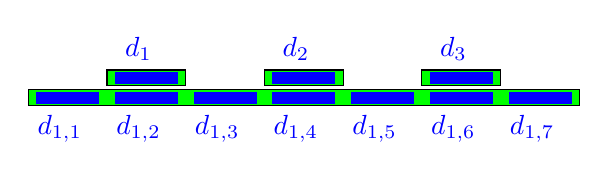
\begin{tikzpicture}[xscale=1,yscale=.25]

\fill[green] (0,2) rectangle (7,2.8);
\draw (0,2) rectangle (7,2.8);

\foreach \x in {1,2,3,4,5,6,7}
{
  \fill[blue] (\x-.9,2.1) rectangle (\x-.1,2.7);
  \node[blue] at (\x-.6,2.0) [below] {$d_{1,\x}$};
}

\foreach \x in {1,2,3}
{
  \fill[green] (2*\x-1,3) rectangle (2*\x-1+1,3.8);
  \draw (2*\x-1,3) rectangle (2*\x-1+1,3.8);
  
  \fill[blue] (2*\x-1+.1,3.1) rectangle (2*\x-1+.9,3.7);
  \node[blue] at (2*\x-1+.4,3.8) [above] {$d_{\x}$};
}

\end{tikzpicture} 
\caption{Simple non-totally unimodular defect set.}
\label{fig:notUni}
\end{figure}

The constraint matrix for the defect set and associated maximal explanations in figure~\ref{fig:notUni} is shown in table~\ref{table:notUni}. We use Camion's necessary and sufficient condition for total unimodularity from \cite{camion1965} to prove this constraint array is not totally unimodular.  We quote that theorem below:

\begin{thm}
Matrix A is totally unimodular if and only if for every (square) Eulerian submatrix $A_j^I \sum_{i\in I} \sum_{j \in J} A^i_j = 0$ mod 4.
\end{thm}

The highlighted cells from our constraint matrix form the following $4 \times 4$ square submatrix:

\begin{tabular}{rrrr}
-1 &  0 &  0 & -1 \\
 0 & -1 &  0 & -1 \\
 0 &  0 & -1 & -1 \\
 1 &  1 &  1 &  1 \\
\end{tabular}  

This submatrix is Eulerian since the sum of elements in each of its rows and columns are even, but the sum of all elements is $-2$, a number that is not divisible by $4$.  By Camion's theorem, this constraint matrix is not totally unimodular, so in general we cannot assume that any of our constraint matrices will be totally unimodular.

\section{Algorithm Bakeoff}

While the only algorithms with calculated bounds are the dynamic programming algorithm, and the Binary Programming algorithm (optimal when a solution is found), we tested our algorithms' performance on randomly generated instances. The algorithms tested were:

\texttt{greedyExplanationCover} The greedy algorithm described in section~\ref{sec:greedy}.  For each of its k steps, places the highest scoring explanation given the explanations already placed.

\texttt{1-OPT} A natural improvement to greedy where the output is improved by a series of single explanation exchanges.  It is greedy itself, choosing the best single exchange at each step and terminating once there are no exchanges that will improve the score.

\texttt{Depth 1 Dynamic Program} The approach from section~\ref{sec:DP}, uses a dynamic program to solve this problem.  The dynamic program's solution is limited to the space of all solutions where no 2 explanations overlap.

\texttt{Depth 2 Dynamic Program} This algorithm, described in section~\ref{sec:dpFixedDepth}, uses a dynamic program to solve this problem.  The dynamic program's solution is limited to the space of all solutions where no 3 explanations overlap.

\texttt{Integer Program Solution} Implements the Binary program from section~\ref{sec:IP} and lets the COIN-OR's OsiClpSolver (as described in \cite{COIN-OR}) use branch and bound methodology to get a solution.

\subsection{Methods}

Because purely random samples are unlikely to find even a local minimum, we modified the GAlib genetic algorithm library \cite{GAlib} to minimize the performance ratios of our algorithms.  A gene consisted of $2N$ integers from $[0,100]$.  Each consecutive pair of endpoints was made into a defect.  

We started with a completely random population, and used a steady state GA with sexual reproduction characterized by two point crossover.  We wrote a custom mutation routine that selected one of the following three randomization operations:

{\it Point flip:} This looped through the entire gene and with constant probability $p$ per endpoint, changed that value to a random number in $[0,100]$.  

{\it Neighbor swap:} Loop through the entire gene, and with probability $p$ per defect, swapped an endpoint of defect $i$ with an endpoint of defect $j$.

{\it Random inversions:} For each position $i$ in the genome, with probability $p$, generate a random number $x$ in $[1,2k-i]$ and reverse the order of the next $x$ alleles.  

We made the objective function to minimize the performance of each algorithm in turn, and ran it for 10,000 generations with a population of 400.  

\subsection{$N=K$ Results}

When $N=K$, the optimal solution would be simply to put one explanation per defect.  This trivial OPT makes these calculations fast.

\begin{tabular}{l|lllll}
{\bf Algo.} & DP 1 & DP 2 & Greedy & 1-OPT  & IP \\ \hline
{\bf $(N,K)$ } \\
(2, 2) & 0.5 & 1 & 0.753 & 1 & 1 \\
(3, 3) & 0.667 & 0.899 & 0.788 & 1 & 1\\
(4, 4) & 0.75 & 0.9 & 0.778 & 1 & 1 \\
(5, 5) & 0.753 & 0.913 & 0.817 & 1 & 1 \\
(6, 6) & 0.774 & 0.907 & 0.819 & 1 & 1 \\
\end{tabular}

\subsection{$N \leq k$}

We then held $N$ steady, and varied $k$. Here we had to use the LP relaxation in place of an {\it a priori } OPT:

\begin{figure}[ht!] \centering
  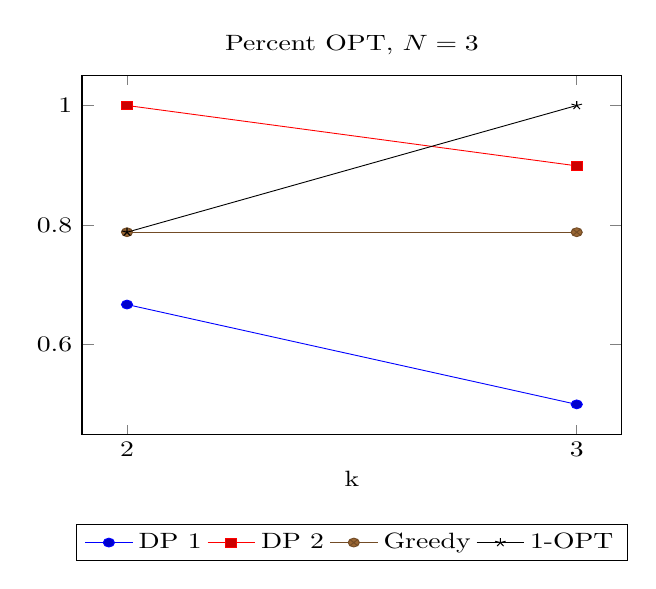
\begin{tikzpicture}[yscale=.8]
    \begin{axis}[ title={Percent OPT, $N=3$}, 
        xlabel=k,
        /pgfplots/xtick={2,...,5},
        legend style={at={(.5,-.25)},anchor=north,legend columns=4},
      ]
      \addplot+[smooth] coordinates {(2, 0.667) (3, 0.5  )};    
      \addplot+[smooth] coordinates {(2, 1.00 ) (3, 0.899)};    
      \addplot+[smooth] coordinates {(2, 0.788) (3, 0.788)};    
      \addplot+[smooth] coordinates {(2, 0.788) (3, 1.0  )};    
      \legend {DP 1, DP 2, Greedy,  1-OPT}
    \end{axis}
  \end{tikzpicture}
  \caption{Results for placing $2-3$ explanations to cover $3$ defects.}
\end{figure}
\FloatBarrier

Here we see what will become the overriding theme.  A one depth dynamic program is strictly inferior to the 2 depth DP, and worst performer overall.  As expected in light of greedy being a preprocessing step to 1-OPT, 1-OPT dominates greedy.  The 2 depth dynamic program outscores 1-OPT for low $k$ and gives up that lead as $k$ increases.

\begin{figure}[ht!] \centering
  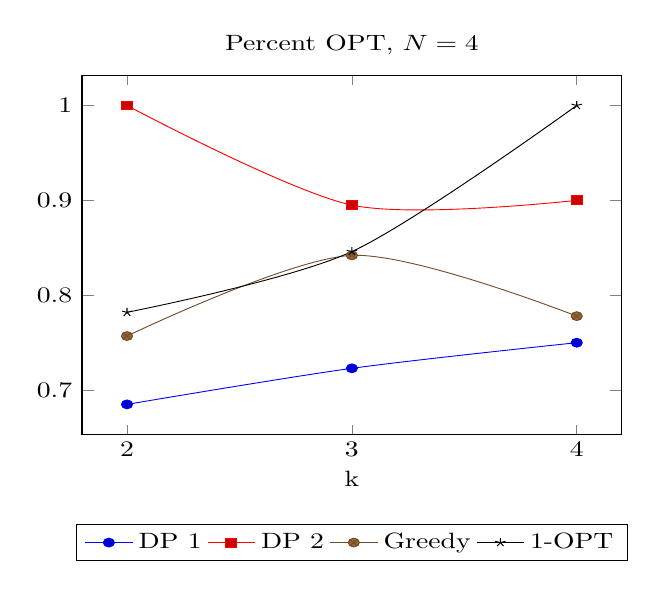
\begin{tikzpicture}[yscale=.8]
    \begin{axis}[ title={Percent OPT, $N=4$}, 
        xlabel=k,
        /pgfplots/xtick={2,...,5},
        legend style={at={(.5,-.25)},anchor=north,legend columns=4},
      ]
      \addplot+[smooth] coordinates {(2, 0.685) (3, 0.723) (4, 0.75 )};    
      \addplot+[smooth] coordinates {(2, 1.00 ) (3, 0.895) (4, 0.9 )};    
      \addplot+[smooth] coordinates {(2, 0.757) (3, 0.842) (4, 0.778 )};    
      \addplot+[smooth] coordinates {(2, 0.782) (3, 0.846) (4, 1.0 )};    
      \legend {DP 1, DP 2, Greedy,  1-OPT}
    \end{axis}
  \end{tikzpicture}
  \caption{Results for placing $2-4$ explanations to cover $4$ defects.}
\end{figure}
\FloatBarrier
The exact same pattern holds, with our algorithms from worst to best being one depth dynamic program, greedy and the 1-OPT / 2 depth tie.

\begin{figure}[ht!] \centering
  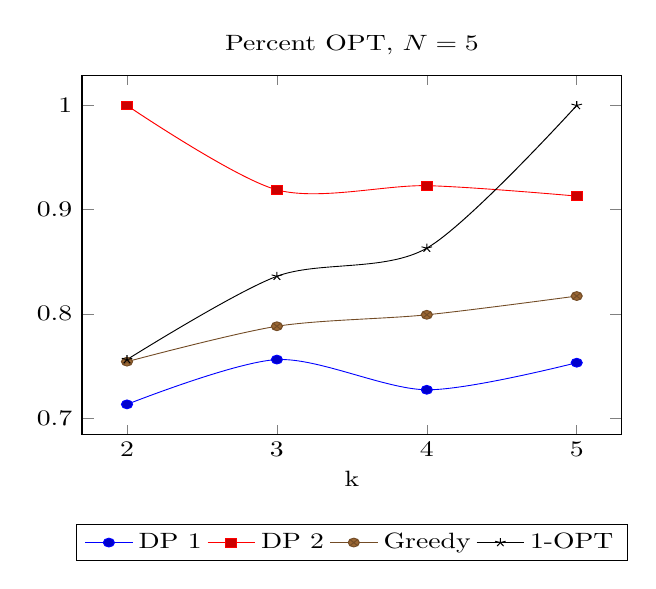
\begin{tikzpicture}[yscale=.8]
    \begin{axis}[ title={Percent OPT, $N=5$}, 
        xlabel=k,
        /pgfplots/xtick={2,...,5},
        legend style={at={(.5,-.25)},anchor=north,legend columns=4},
      ]
      \addplot+[smooth] coordinates {(2, 0.713) (3, 0.756) (4, 0.727) (5,0.753)};    
      \addplot+[smooth] coordinates {(2, 1.00 ) (3, 0.919) (4, 0.923) (5, 0.913)};    
      \addplot+[smooth] coordinates {(2, 0.754) (3, 0.788) (4, 0.799) (5,0.817)};    
      \addplot+[smooth] coordinates {(2, 0.756) (3, 0.836) (4, 0.863) (5,1) };    
      \legend {DP 1, DP 2, Greedy,  1-OPT}
    \end{axis}
  \end{tikzpicture}
  \caption{Results for placing $2-5$ explanations to cover $5$ defects.}
\end{figure}
\FloatBarrier
Here, while the rankings don't change, the 2-depth dynamic program held its lead for all but the $N=K$ case.  Considering that 1-OPT will always find the optimal solution in an $N=k$ case, and that real life scenarios are characterized by $N>>k$, this result strongly suggests that the 2 depth dynamic program outperforms the other three heuristics.  

The clear winner was binary programming (not shown).  In all but 4 of the genome evaluations (out of ~1.6 million), the MILP solver from COIN-OR produced an optimal output.  If it scales well for problems of real world applicationsize, it would be the best algorithm to use in practice.

\FloatBarrier

\subsection{Timing Data}

To illustrate algorithm running times on smallscale problems, we generated 1024 random defect sets of size $N \in \{4 8 16\}$ and had each algorithm place $K = \{ N, N/2, N/4\}$ explanations.  The timing results follow:

\begin{figure}[ht!] \centering
  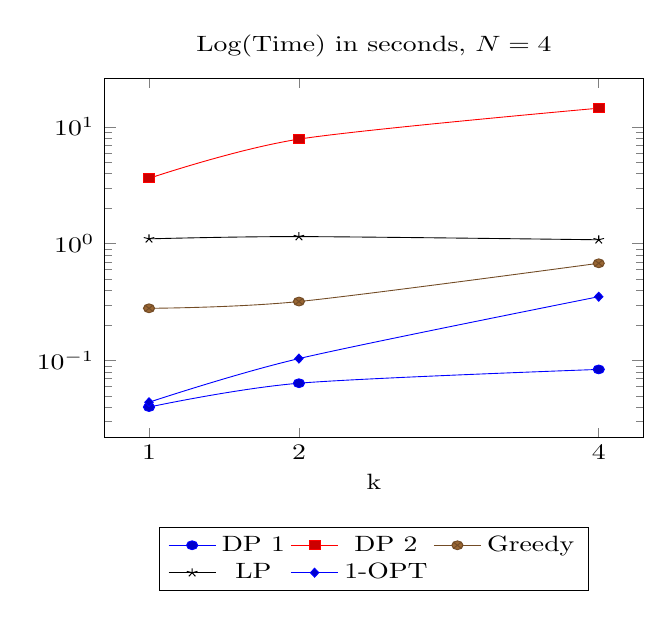
\begin{tikzpicture}[yscale=.8]
    \begin{axis}[ title={Log(Time) in seconds, $N=4$}, 
        ymode=log,
        xlabel=k,
        /pgfplots/xtick={1,2,4},
        legend style={at={(.5,-.25)},anchor=north,legend columns=3},
      ]
      \addplot+[smooth] coordinates {(1, 0.04) (2, 0.064) (4, 0.084) };    
      \addplot+[smooth] coordinates {(1, 3.624) (2, 7.848 ) (4, 14.436) };    
      \addplot+[smooth] coordinates {(1, 0.28) (2,0.32 ) (4,0.68 ) };    
      \addplot+[smooth] coordinates {(1, 1.1 ) (2,1.15 ) (4,1.08 ) };    
      \addplot+[smooth] coordinates {(1, .044) (2, .104) (4, .352 ) };    
      \legend {DP 1, DP 2, Greedy,  LP, 1-OPT}
    \end{axis}
  \end{tikzpicture}
  \caption{Time to place $k$ explanations to cover 4 defects.}
\end{figure}
\FloatBarrier

Even for small cases, the depth 2 dynamic program is more than 10 times slower than any other algorithm.  Since it scales as $O(kn^{2+k})$, this algorithm will quickly become impractical.  We will devote a chart to its scaling, but omit it from the rest of the timing plots.

\begin{figure}[ht!] \centering
  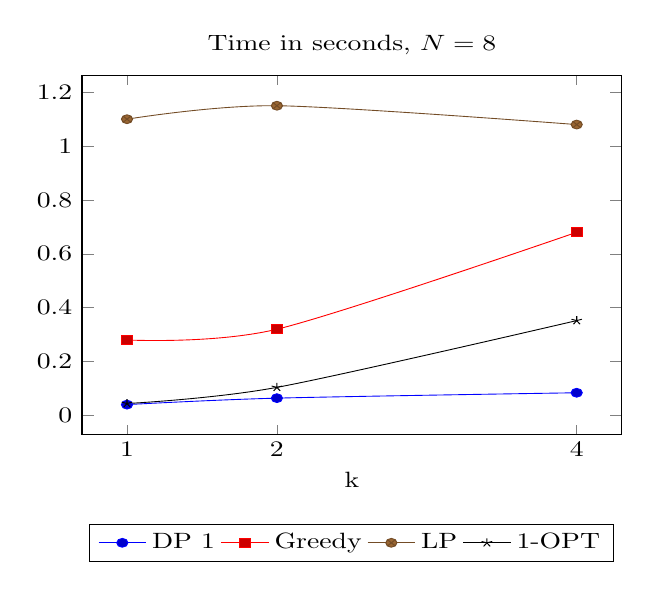
\begin{tikzpicture}[yscale=.8]
    \begin{axis}[ title={Time in seconds, $N=8$}, 
        xlabel=k,
        /pgfplots/xtick={1,2,4},
        legend style={at={(.5,-.25)},anchor=north,legend columns=4},
      ]
      \addplot+[smooth] coordinates {(1, 0.04) (2, 0.064) (4, 0.084) };    
      \addplot+[smooth] coordinates {(1, 0.28) (2,0.32 ) (4,0.68 ) };    
      \addplot+[smooth] coordinates {(1, 1.1 ) (2,1.15 ) (4,1.08 ) };    
      \addplot+[smooth] coordinates {(1, .044) (2, .104) (4, .352 ) };    
      \legend {DP 1, Greedy,  LP, 1-OPT}
    \end{axis}
  \end{tikzpicture}
  \caption{Time to place $k$ explanations to cover 8 defects.}
\end{figure}

\begin{figure}[ht!] \centering
  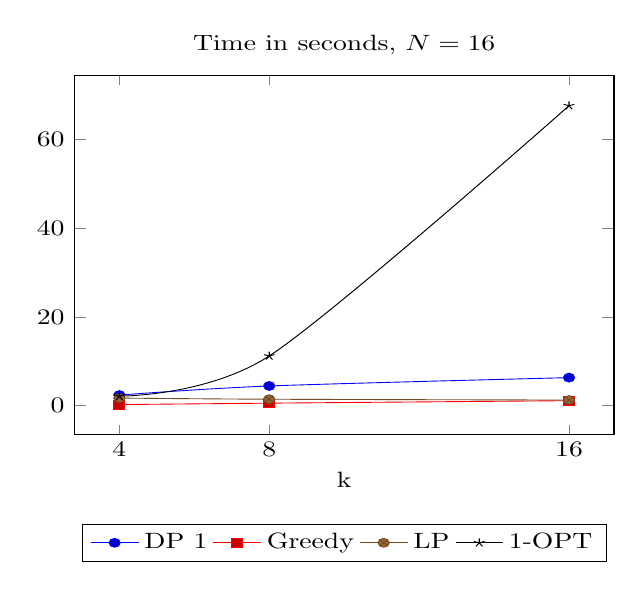
\begin{tikzpicture}[yscale=.8]
    \begin{axis}[ title={Time in seconds, $N=16$}, 
        xlabel=k,
        /pgfplots/xtick={4,8,16},
        legend style={at={(.5,-.25)},anchor=north,legend columns=4},
      ]
      \addplot+[smooth] coordinates {(4, 2.39) (8,4.44 ) (16,6.32 ) };    
      \addplot+[smooth] coordinates {(4,0.244 ) (8,0.568 ) (16,1.126 ) };    
      \addplot+[smooth] coordinates {(4,1.716 ) (8,1.456 ) (16,1.272 ) };    
      \addplot+[smooth] coordinates {(4,2.15 ) (8,11.2 ) (16,67.6 ) };    
      \legend {DP 1, Greedy,  LP, 1-OPT}
    \end{axis}
  \end{tikzpicture}
  \caption{Time to place $k$ explanations to cover 16 defects.}
\end{figure}

\begin{figure}[ht!] \centering
  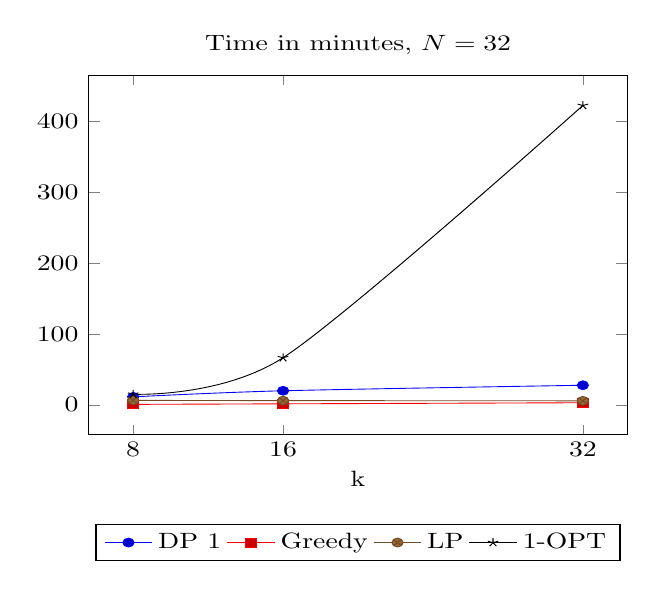
\begin{tikzpicture}[yscale=.8]
    \begin{axis}[ title={Time in minutes, $N=32$}, 
        xlabel=k,
        /pgfplots/xtick={8,16, 32},
        legend style={at={(.5,-.25)},anchor=north,legend columns=4},
      ]
      \addplot+[smooth] coordinates {(8,11.2 ) (16,19.8 ) (32,27.6) };    
      \addplot+[smooth] coordinates {(8,0.6 ) (16,1.35 ) (32,2.9) };    
      \addplot+[smooth] coordinates {(8,6.25 ) (16,5.9) (32,5.6) };    
      \addplot+[smooth] coordinates {(8,14.9 ) (16,66.5 ) (32,422.75) };    
      \legend {DP 1, Greedy,  LP, 1-OPT}
    \end{axis}
  \end{tikzpicture}
  \caption{Time to place $k$ explanations to cover 32 defects.}
\end{figure}

\FloatBarrier

A log-log linear regression on the $k$ dependence of the 1-OPT algorithm shows that its dependence on $k$ is approximately $O(k^{2.5})$.  For moderate values of $k\leq 100$, this may prove acceptable for use in the field. 


\subsubsection{2-Depth DP Timing}

\begin{figure}[ht!] \centering
  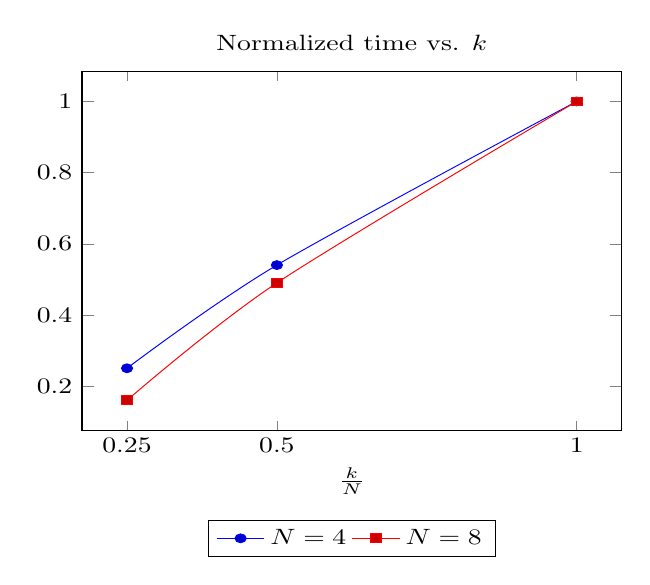
\begin{tikzpicture}[yscale=.8]
    \begin{axis}[ title={Normalized time vs. $k$}, 
        xlabel=$\frac{k}{N}$,
        /pgfplots/xtick={.25,.5,1},
        legend style={at={(.5,-.25)},anchor=north,legend columns=2},
      ]
      \addplot+[smooth] coordinates {(.25,0.25) (.5,0.54) (1,1) };    
      \addplot+[smooth] coordinates {(.25,0.16) (.5,0.49) (1,1) };    
      \legend {$N=4$, $N=8$}
    \end{axis}
  \end{tikzpicture}
  \caption{Timing data for the 2-depth dynamic program. Note that time is normalized by the duration of the $N=k$ call.}
\end{figure}

The running time dependence on $k$ for the 2-Depth dynamic program is exactly as it should be: linear.

\begin{figure}[ht!] \centering
  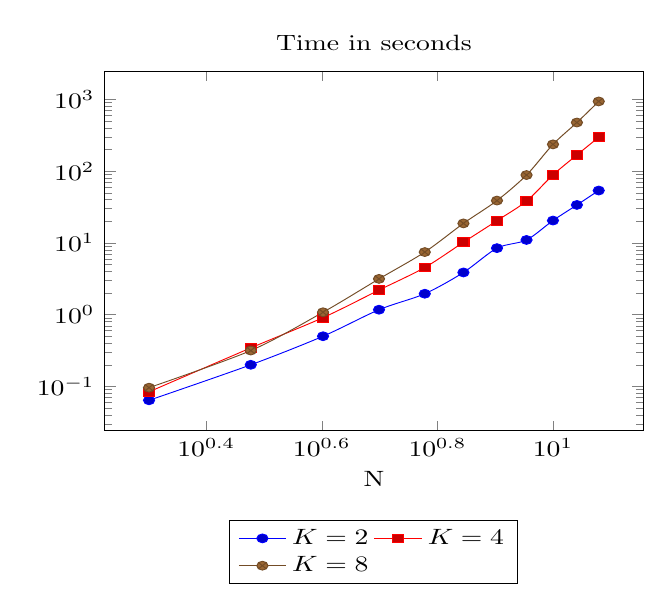
\begin{tikzpicture}[yscale=.8]
    \begin{axis}[ title={Time in seconds}, 
        xlabel=N,
        ymode=log,
        xmode=log,
        legend style={at={(.5,-.25)},anchor=north,legend columns=2},
      ]
      \addplot+[smooth] coordinates {(2, 0.064) (3, 0.200) (4, 0.500) (5, 1.172) (6, 1.956) (7, 3.872) (8, 8.448) (9, 10.992) (10, 20.5) (11, 33.8) (12, 53.7)};
      \addplot+[smooth] coordinates {(2, 0.084) (3, 0.344) (4, 0.908) (5, 2.2) (6, 4.54) (7, 10.2) (8, 20.4) (9, 38.3) (10, 88.6) (11, 168) (12, 297)};
      \addplot+[smooth] coordinates {(2, 0.096) (3, 0.316) (4, 1.08) (5, 3.15) (6, 7.45) (7, 18.7) (8, 38.9) (9, 88.3) (10, 236) (11, 476) (12, 937)};
    \legend {$K=2$, $K=4$, $K=8$}
    \end{axis}
  \end{tikzpicture}
  \caption{Timing data for the 2-depth dynamic program as a function of $N$}
\end{figure}

On the other hand, the pessimistic $O(kN^{k+2})$ upper bound on running time is exactly that, pessimistic. The best fitting line's slope for the log-log plot with $k=2$ was 3.78, and for $k=4$ it was 4.26, and 5.21 for $k=8$. We hypothesize that they are below the pessimistic $4, 6$ and $10$, because that bound would require our defect set be of depth $O(N)$ for the majority of times we encounter an endpoint. 

If this hypothesis holds, it's possible that the structure of real data will allow for even better running times for the dynamic programming algorithm than did our synthetic data.

\FloatBarrier
\section{Conclusions}

We studied a number of candidate heuristics for the DNA copy number analysis problem.  Our most powerful approaches were a binary programming formuation of the problem and dynamic programming based PTAS. The PTAS has both a stronger theoretical grounding and performance guarantees, but its running time is prohibitively expensive.

Fortunately, the binary programming formulation solved with a freeware MILP had a very acceptable running time for problems of modest size.  It is our recommendation that researchers, specifically those who implemented the CORE product referenced in \cite{krasnitz2013target}, utilize this optimization method in place of their current greedy approach.
